\documentclass[11pt]{articulo}
%%%\documentclass[12pt]{articulo}
\usepackage{amsmath}
\usepackage{graphicx}

\baselineskip 25pt
\textwidth 15cm
\textheight 23cm
\topmargin -1.5cm
\oddsidemargin 1cm 
\evensidemargin 1cm 

\begin{document}

\title{\bf Laboratorio de F\'isica I\\
  Gu\'ia del experimento Aerodin\'amica} 
\author{
  {\bf J\'onatan Piedra}\\
  Universidad de Cantabria}
\maketitle


\section{Introducci\'on}

En esta pr\'actica se estudiar\'an experimentalmente los principios b\'asicos de la din\'amica de fluidos (ecuaci\'on de Bernoulli) y del vuelo. En un t\'unel aerodin\'amico de secci\'on variable se medir\'an la presi\'on total y el caudal para varias secciones. Se medir\'a la fuerza de elevaci\'on sobre un perfil de ala para varias velocidades del aire. Tambi\'en se estimar\'a esta fuerza a partir de las medidas de la presi\'on en las partes superior e inferior del perfil.


\section{Fundamento te\'orico}

\subsection{Ecuaci\'on de Bernoulli}

Para la realizaci\'on de esta pr\'actica se debe tener claro el concepto de presi\'on, as\'i como las ideas b\'asicas de la din\'amica de fluidos, en particular la ecuaci\'on de Bernoulli~\cite{tipler}. Esta ecuaci\'on establece que a lo largo de una l\'inea de corriente de un fluido incompresible y sin viscosidad, la suma de las presiones est\'atica $p$, hidrost\'atica $\rho g z$, y din\'amica $\rho v^2/2$, es constante,
%
\begin{equation*}
p + \rho g z + \rho \frac{v^2}{2} = p_t = {\rm constante},
\end{equation*}
%
donde $\rho$ es la densidad del fluido, $v$ la velocidad, $z$ la altura y $p_t$ la presi\'on total. Si la altura es constante se obtiene
%
\begin{equation*}
p + \rho \frac{v^2}{2} = p_t = {\rm constante},
\end{equation*}
%
y entonces se puede obtener el valor de la velocidad partir de las presiones total y est\'atica.

\subsection{Vuelo}

Cuando un cuerpo se mueve respecto al aire aparecen dos fuerzas, una perpendicular (elevaci\'on, $F_e$) y otra paralela (arrastre, $F_a$) a la velocidad del aire. El origen de estas fuerzas se puede entender a partir de las leyes de Newton~\cite{anderson}. Debido a la viscosidad del aire su velocidad en la superficie del ala es nula. Como consecuencia las l\'ineas de corriente del aire se doblan siguiendo la superficie del ala, por lo que el aire se mueve hacia abajo cuando el \'angulo del ala con la direcci\'on del viento, conocido como \'angulo de ataque (Figura~\ref{aerofoil} izquierda), es positivo (Figura~\ref{aerofoil} centro~\cite{babinsky}). Como reacci\'on aparece una fuerza sobre el ala dada por $vdm/dt$, donde $m$ es la masa de aire desviada hacia abajo y $v$ es la velocidad. Esta fuerza es proporcional a $\rho v^2S$, donde $\rho$ es la densidad del aire y $S$ es la superficie del ala.

\begin{figure}[htb]
\begin{center}
\hspace*{0.0cm}
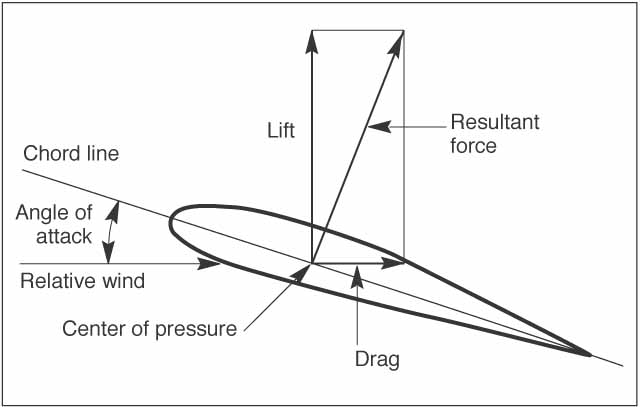
\includegraphics[width=0.332\textwidth]{figuras/aerodinamica_Figura_1a.jpg}
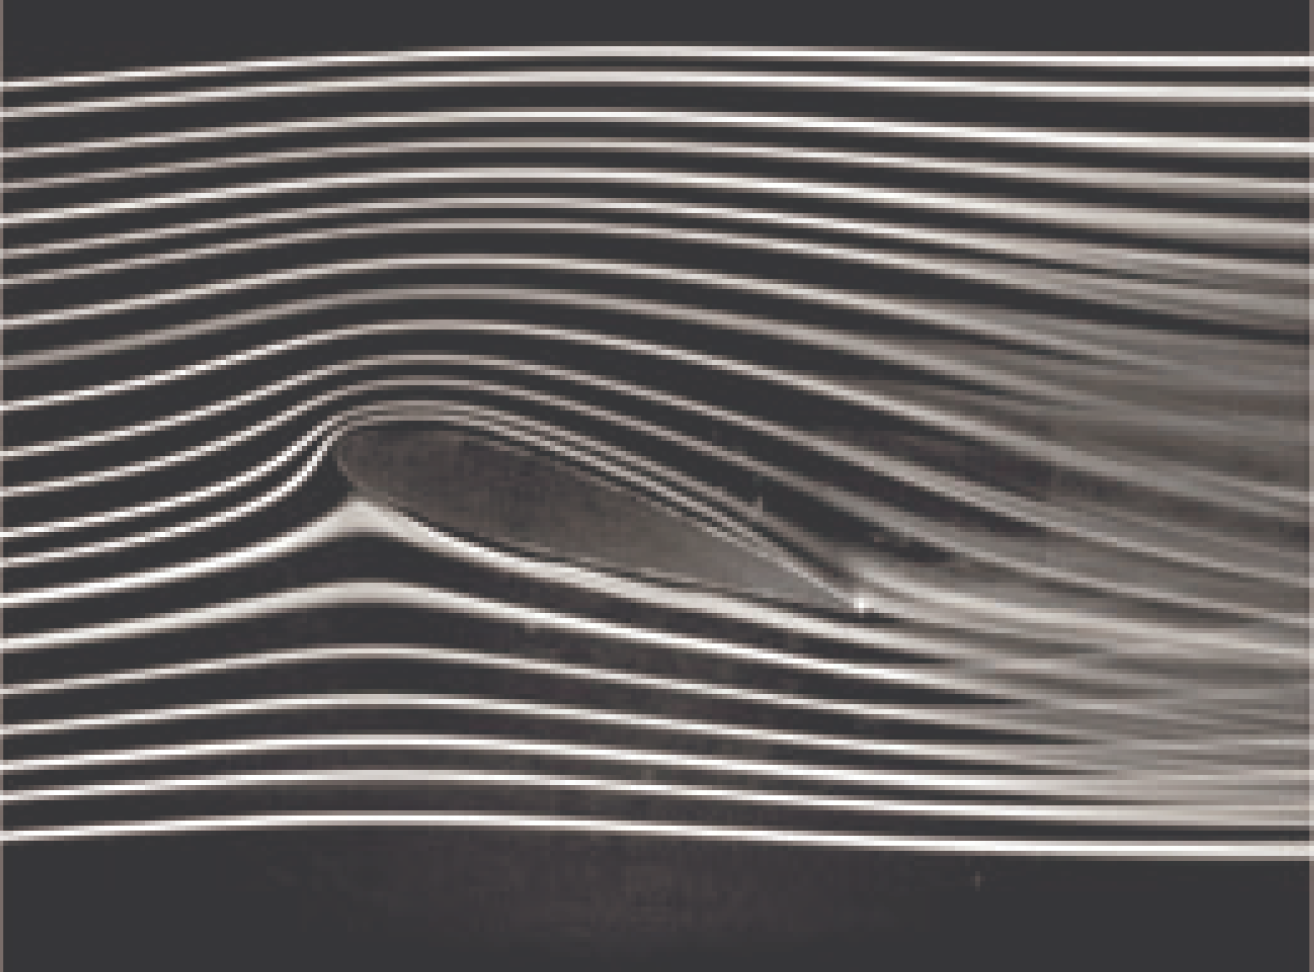
\includegraphics[width=0.284\textwidth]{figuras/aerodinamica_Figura_1b.png}
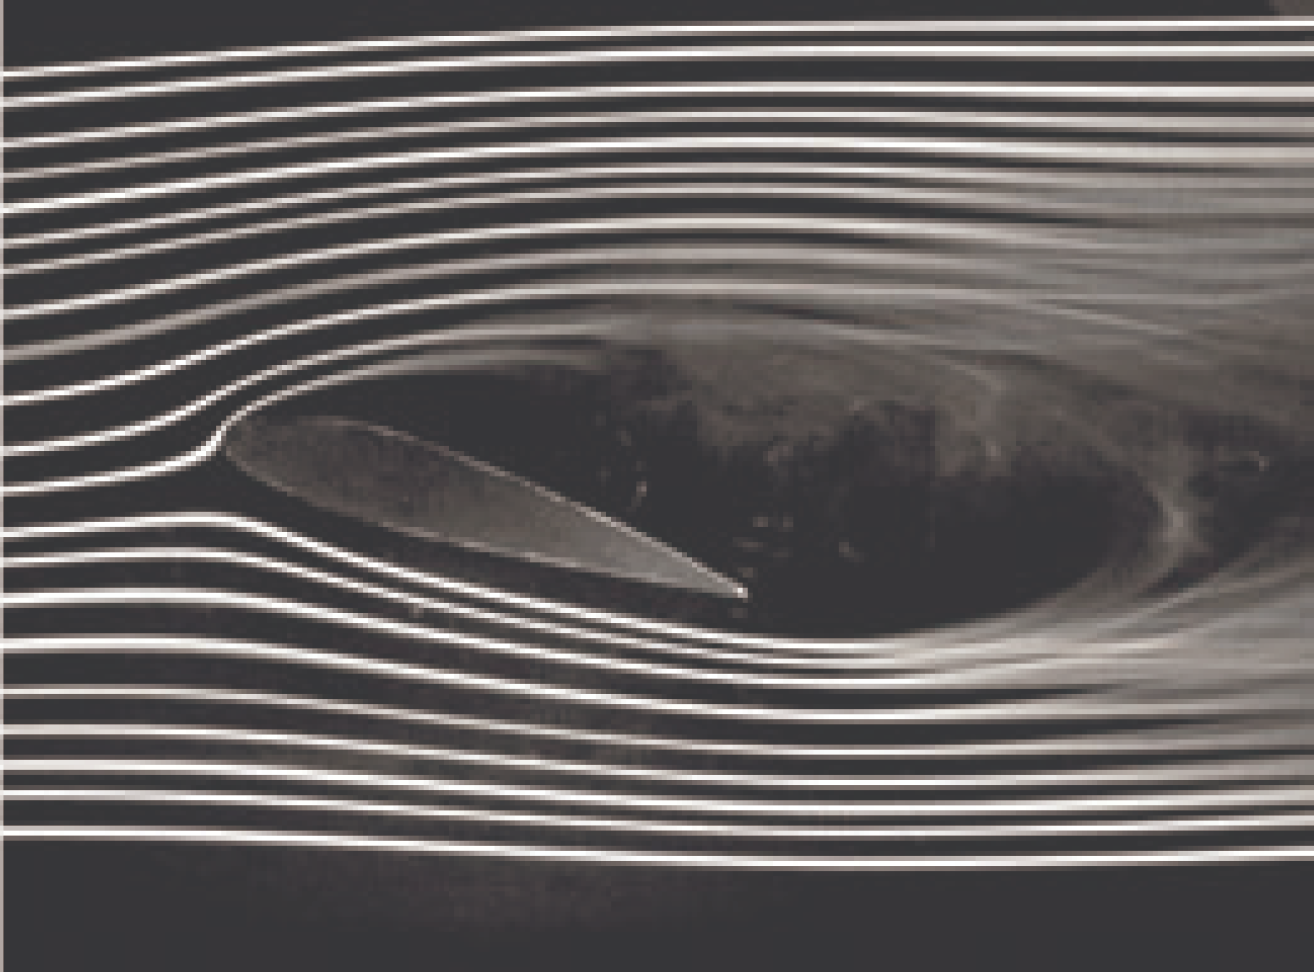
\includegraphics[width=0.284\textwidth]{figuras/aerodinamica_Figura_1c.png}
\end{center}
\vspace*{-0.6cm}
\caption[]{\label{aerofoil}{\'Angulo de ataque (izquierda). Las l\'ineas de corriente del aire siguen la superficie del ala (centro). Las l\'ineas de corriente del aire no siguen la superficie del ala, entrando en turbulencia (derecha).}}
\end{figure}

Para \'angulos de ataque peque\~nos


%-------------------------------------------------------------------------------
% Bibliografia
%-------------------------------------------------------------------------------

\begin{thebibliography}{X}

\bibitem{tipler}
P.~A.~Tipler y G.~Mosca,
\textit{F\'isica para la ciencia y la tecnolog\'ia}. 
Editorial Revert\'e, 2005, $5^{a}$ edici\'on, Volumen 1, Cap\'itulo 13.

\bibitem{anderson}
D.~F.~Anderson, S.~Eberhardt,
\textit{The Newtonian description of lift of a wing}.
FERMILAB-Pub-01/036-E, 2001.

\bibitem{babinsky}
H.~Babinsky,
{\it How do wings work?}
Physics Education {\bf 38}, pp. 497-503, 2003.

\end{thebibliography}


%-------------------------------------------------------------------------------
% Fin del documento
%-------------------------------------------------------------------------------

\end{document}
